\chapter{強連結 - Strong connectivity}

\index{強連結グラフ - strongly connected graph}

有向グラフは辺は一方向にしか進めないのでために、
あるグラフ上のあるノードから別のノードへの経路が存在することは保証されません。
そこでノードとノードに辺があるとは違う新しい概念の定義に意味があります。

グラフ内の任意のノードから他のすべてのノードへのパスが存在する場合、
グラフは\key{強連結 - strongly connected}であるといいます。
次の図では左のグラフは強連結ですが右のグラフは強連結ではありません。

\begin{center}
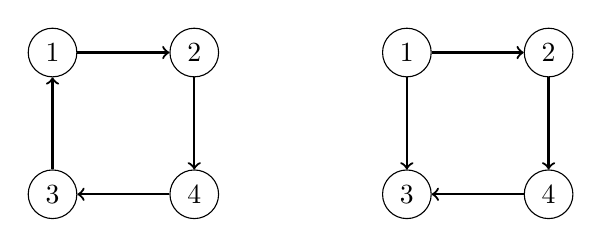
\begin{tikzpicture}[scale=0.9]
\node[draw, circle] (1) at (1,1) {$1$};
\node[draw, circle] (2) at (3,1) {$2$};
\node[draw, circle] (3) at (1,-1) {$3$};
\node[draw, circle] (4) at (3,-1) {$4$};

\path[draw,thick,->] (1) -- (2);
\path[draw,thick,->] (2) -- (4);
\path[draw,thick,->] (4) -- (3);
\path[draw,thick,->] (3) -- (1);

\node[draw, circle] (1b) at (6,1) {$1$};
\node[draw, circle] (2b) at (8,1) {$2$};
\node[draw, circle] (3b) at (6,-1) {$3$};
\node[draw, circle] (4b) at (8,-1) {$4$};

\path[draw,thick,->] (1b) -- (2b);
\path[draw,thick,->] (2b) -- (4b);
\path[draw,thick,->] (4b) -- (3b);
\path[draw,thick,->] (1b) -- (3b);
\end{tikzpicture}
\end{center}

具体的には、右のグラフは2から1へ到達できないために強連結グラフといえません。

\index{強連結成分 - strongly connected component}
\index{成分グラフ - component graph}

\key{強連結成分 - strongly connected components}は、
グラフをできるだけ大きな強連結な部分である成分グラフで、
元のグラフの閉路を含まない成分グラフから形成されます。

\begin{center}
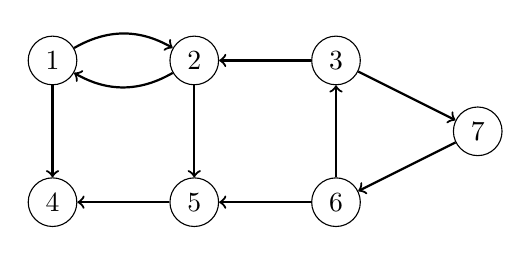
\begin{tikzpicture}[scale=0.9,label distance=-2mm]
\node[draw, circle] (1) at (-1,1) {$7$};
\node[draw, circle] (2) at (-3,2) {$3$};
\node[draw, circle] (4) at (-5,2) {$2$};
\node[draw, circle] (6) at (-7,2) {$1$};
\node[draw, circle] (3) at (-3,0) {$6$};
\node[draw, circle] (5) at (-5,0) {$5$};
\node[draw, circle] (7) at (-7,0) {$4$};

\path[draw,thick,->] (2) -- (1);
\path[draw,thick,->] (1) -- (3);
\path[draw,thick,->] (3) -- (2);
\path[draw,thick,->] (2) -- (4);
\path[draw,thick,->] (3) -- (5);
\path[draw,thick,->] (4) edge [bend left] (6);
\path[draw,thick,->] (6) edge [bend left] (4);
\path[draw,thick,->] (4) -- (5);
\path[draw,thick,->] (5) -- (7);
\path[draw,thick,->] (6) -- (7);
\end{tikzpicture}
\end{center}
強連結成分は以下のようになります。
\begin{center}
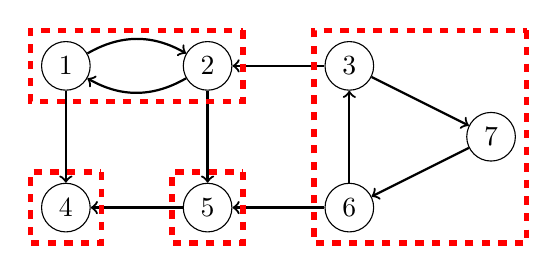
\begin{tikzpicture}[scale=0.9]
\node[draw, circle] (1) at (-1,1) {$7$};
\node[draw, circle] (2) at (-3,2) {$3$};
\node[draw, circle] (4) at (-5,2) {$2$};
\node[draw, circle] (6) at (-7,2) {$1$};
\node[draw, circle] (3) at (-3,0) {$6$};
\node[draw, circle] (5) at (-5,0) {$5$};
\node[draw, circle] (7) at (-7,0) {$4$};

\path[draw,thick,->] (2) -- (1);
\path[draw,thick,->] (1) -- (3);
\path[draw,thick,->] (3) -- (2);
\path[draw,thick,->] (2) -- (4);
\path[draw,thick,->] (3) -- (5);
\path[draw,thick,->] (4) edge [bend left] (6);
\path[draw,thick,->] (6) edge [bend left] (4);
\path[draw,thick,->] (4) -- (5);
\path[draw,thick,->] (5) -- (7);
\path[draw,thick,->] (6) -- (7);

\draw [red,thick,dashed,line width=2pt] (-0.5,2.5) rectangle (-3.5,-0.5);
\draw [red,thick,dashed,line width=2pt] (-4.5,2.5) rectangle (-7.5,1.5);
\draw [red,thick,dashed,line width=2pt] (-4.5,0.5) rectangle (-5.5,-0.5);
\draw [red,thick,dashed,line width=2pt] (-6.5,0.5) rectangle (-7.5,-0.5);
\end{tikzpicture}
\end{center}
これに対応する成分グラフは次の通りとなります。
\begin{center}
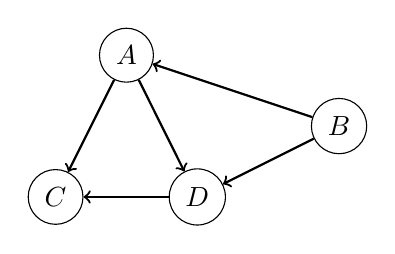
\begin{tikzpicture}[scale=0.9]
\node[draw, circle] (1) at (-3,1) {$B$};
\node[draw, circle] (2) at (-6,2) {$A$};
\node[draw, circle] (3) at (-5,0) {$D$};
\node[draw, circle] (4) at (-7,0) {$C$};

\path[draw,thick,->] (1) -- (2);
\path[draw,thick,->] (1) -- (3);
\path[draw,thick,->] (2) -- (3);
\path[draw,thick,->] (2) -- (4);
\path[draw,thick,->] (3) -- (4);
\end{tikzpicture}
\end{center}
ここでの成分は $A=\{1,2\}$,
$B=\{3,6,7\}$, $C=\{4\}$, $D=\{5\}$となります。

この成分グラフは閉路を含まない有向グラフであるため、
元のグラフよりも処理しやすくなります。
閉路が含まれないので確実にトポロジカルソートの操作ができ、
16章で紹介したのような動的計画法を利用することができます。

\section{Kosaraju's algorithm}

\index{Kosaraju's algorithm}

\key{Kosaraju's algorithm}\footnote{According to \cite{aho83},
S. R. Kosaraju invented this algorithm in 1978
but did not publish it. In 1981, the same algorithm was rediscovered
and published by M. Sharir \cite{sha81}.}
は有向グラフの強連結成分を効率的に求める方法です。
このアルゴリズムでは、2回の深さ優先探索を行います。
1回目の探索で探索でグラ フの構造に従ってノードのリストを構築し、
2回目の探索で強連結成分を求めます。

\subsubsection{1回目の探索 - Search 1}

まず、深さ優先探索が処理する順番にノードのリストを構築します。
未処理の 各ノードで深さ優先探索をし、リストに追加します。
このグラフの例では、以下の順序でノードが処理されていきます。

\begin{center}
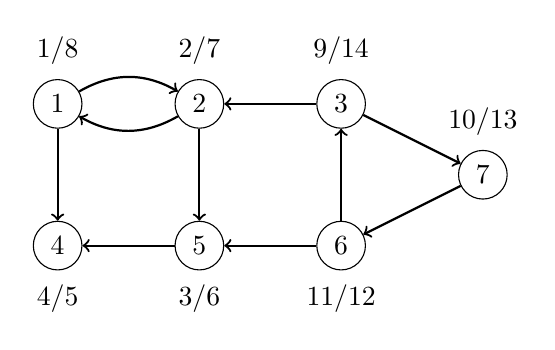
\begin{tikzpicture}[scale=0.9,label distance=-2mm]
\node[draw, circle] (1) at (-1,1) {$7$};
\node[draw, circle] (2) at (-3,2) {$3$};
\node[draw, circle] (4) at (-5,2) {$2$};
\node[draw, circle] (6) at (-7,2) {$1$};
\node[draw, circle] (3) at (-3,0) {$6$};
\node[draw, circle] (5) at (-5,0) {$5$};
\node[draw, circle] (7) at (-7,0) {$4$};

\node at (-7,2.75) {$1/8$};
\node at (-5,2.75) {$2/7$};
\node at (-3,2.75) {$9/14$};
\node at (-7,-0.75) {$4/5$};
\node at (-5,-0.75) {$3/6$};
\node at (-3,-0.75) {$11/12$};
\node at (-1,1.75) {$10/13$};

\path[draw,thick,->] (2) -- (1);
\path[draw,thick,->] (1) -- (3);
\path[draw,thick,->] (3) -- (2);
\path[draw,thick,->] (2) -- (4);
\path[draw,thick,->] (3) -- (5);
\path[draw,thick,->] (4) edge [bend left] (6);
\path[draw,thick,->] (6) edge [bend left] (4);
\path[draw,thick,->] (4) -- (5);
\path[draw,thick,->] (5) -- (7);
\path[draw,thick,->] (6) -- (7);
\end{tikzpicture}
\end{center}

$x/y$という表記は$x$に探索が始まり、$y$に探索が終わったことを示します。

\begin{tabular}{ll}
\\
ノード番号 & 処理完了時間 \\
\hline
4 & 5 \\
5 & 6 \\
2 & 7 \\
1 & 8 \\
6 & 12 \\
7 & 13 \\
3 & 14 \\
\\
\end{tabular}
%
% In the second phase of the algorithm,
% the nodes will be processed
% in reverse order: $[3,7,6,1,2,5,4]$.

\subsubsection{2回目の探索 - Search 2}

次に強連結成分を求めていきます。
まず、グラフのすべてのエッジを逆向きに反転させます。
これによって、余分なノードを持たない強連結成分を必ず見つけることが保証されます。
辺を反転させると次のようなグラフになります。

\begin{center}
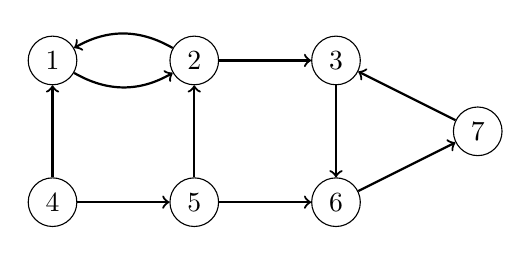
\begin{tikzpicture}[scale=0.9,label distance=-2mm]
\node[draw, circle] (1) at (-1,1) {$7$};
\node[draw, circle] (2) at (-3,2) {$3$};
\node[draw, circle] (4) at (-5,2) {$2$};
\node[draw, circle] (6) at (-7,2) {$1$};
\node[draw, circle] (3) at (-3,0) {$6$};
\node[draw, circle] (5) at (-5,0) {$5$};
\node[draw, circle] (7) at (-7,0) {$4$};

\path[draw,thick,<-] (2) -- (1);
\path[draw,thick,<-] (1) -- (3);
\path[draw,thick,<-] (3) -- (2);
\path[draw,thick,<-] (2) -- (4);
\path[draw,thick,<-] (3) -- (5);
\path[draw,thick,<-] (4) edge [bend left] (6);
\path[draw,thick,<-] (6) edge [bend left] (4);
\path[draw,thick,<-] (4) -- (5);
\path[draw,thick,<-] (5) -- (7);
\path[draw,thick,<-] (6) -- (7);
\end{tikzpicture}
\end{center}

この後、
最初の検索で作成されたノードのリストを逆順に捜査します。
ノードが成分に属さない場合、
新しい成分を作成してその探索中に見つかったすべての新しいノードを
新しい成分に追加する深さ優先探索を行います。
このグラフの例では、最初のコンポーネントはノード3から始まっています
(最初の探索で最後のノードは3だったことを思い出してください)。

\begin{center}
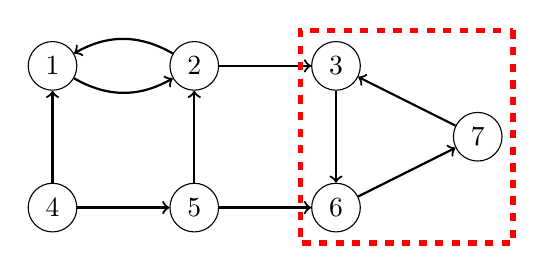
\begin{tikzpicture}[scale=0.9,label distance=-2mm]
\node[draw, circle] (1) at (-1,1) {$7$};
\node[draw, circle] (2) at (-3,2) {$3$};
\node[draw, circle] (4) at (-5,2) {$2$};
\node[draw, circle] (6) at (-7,2) {$1$};
\node[draw, circle] (3) at (-3,0) {$6$};
\node[draw, circle] (5) at (-5,0) {$5$};
\node[draw, circle] (7) at (-7,0) {$4$};

\path[draw,thick,<-] (2) -- (1);
\path[draw,thick,<-] (1) -- (3);
\path[draw,thick,<-] (3) -- (2);
\path[draw,thick,<-] (2) -- (4);
\path[draw,thick,<-] (3) -- (5);
\path[draw,thick,<-] (4) edge [bend left] (6);
\path[draw,thick,<-] (6) edge [bend left] (4);
\path[draw,thick,<-] (4) -- (5);
\path[draw,thick,<-] (5) -- (7);
\path[draw,thick,<-] (6) -- (7);

\draw [red,thick,dashed,line width=2pt] (-0.5,2.5) rectangle (-3.5,-0.5);
\end{tikzpicture}
\end{center}

全てのグラフは反転しているため、成分が他の成分にリークすることはありません。

\begin{samepage}
リストの次のノードは$7$と$6$ですが、
これらは既に成分に属しているのでこの成分の探索は完了します。
次にノード1から新しい成分の探索を開始します。

\begin{center}
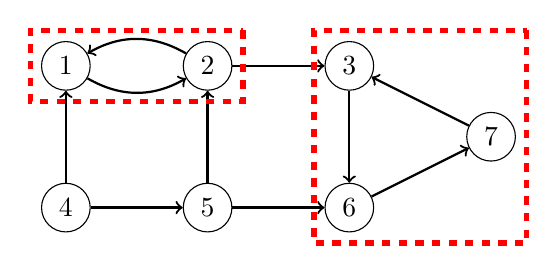
\begin{tikzpicture}[scale=0.9,label distance=-2mm]
\node[draw, circle] (1) at (-1,1) {$7$};
\node[draw, circle] (2) at (-3,2) {$3$};
\node[draw, circle] (4) at (-5,2) {$2$};
\node[draw, circle] (6) at (-7,2) {$1$};
\node[draw, circle] (3) at (-3,0) {$6$};
\node[draw, circle] (5) at (-5,0) {$5$};
\node[draw, circle] (7) at (-7,0) {$4$};

\path[draw,thick,<-] (2) -- (1);
\path[draw,thick,<-] (1) -- (3);
\path[draw,thick,<-] (3) -- (2);
\path[draw,thick,<-] (2) -- (4);
\path[draw,thick,<-] (3) -- (5);
\path[draw,thick,<-] (4) edge [bend left] (6);
\path[draw,thick,<-] (6) edge [bend left] (4);
\path[draw,thick,<-] (4) -- (5);
\path[draw,thick,<-] (5) -- (7);
\path[draw,thick,<-] (6) -- (7);

\draw [red,thick,dashed,line width=2pt] (-0.5,2.5) rectangle (-3.5,-0.5);
\draw [red,thick,dashed,line width=2pt] (-4.5,2.5) rectangle (-7.5,1.5);
%\draw [red,thick,dashed,line width=2pt] (-4.5,0.5) rectangle (-5.5,-0.5);
%\draw [red,thick,dashed,line width=2pt] (-6.5,0.5) rectangle (-7.5,-0.5);
\end{tikzpicture}
\end{center}
\end{samepage}

\begin{samepage}

同じように次の成分として5。そして4が処理されます。

\begin{center}
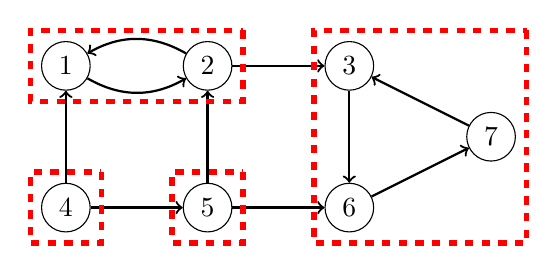
\begin{tikzpicture}[scale=0.9,label distance=-2mm]
\node[draw, circle] (1) at (-1,1) {$7$};
\node[draw, circle] (2) at (-3,2) {$3$};
\node[draw, circle] (4) at (-5,2) {$2$};
\node[draw, circle] (6) at (-7,2) {$1$};
\node[draw, circle] (3) at (-3,0) {$6$};
\node[draw, circle] (5) at (-5,0) {$5$};
\node[draw, circle] (7) at (-7,0) {$4$};

\path[draw,thick,<-] (2) -- (1);
\path[draw,thick,<-] (1) -- (3);
\path[draw,thick,<-] (3) -- (2);
\path[draw,thick,<-] (2) -- (4);
\path[draw,thick,<-] (3) -- (5);
\path[draw,thick,<-] (4) edge [bend left] (6);
\path[draw,thick,<-] (6) edge [bend left] (4);
\path[draw,thick,<-] (4) -- (5);
\path[draw,thick,<-] (5) -- (7);
\path[draw,thick,<-] (6) -- (7);

\draw [red,thick,dashed,line width=2pt] (-0.5,2.5) rectangle (-3.5,-0.5);
\draw [red,thick,dashed,line width=2pt] (-4.5,2.5) rectangle (-7.5,1.5);
\draw [red,thick,dashed,line width=2pt] (-4.5,0.5) rectangle (-5.5,-0.5);
\draw [red,thick,dashed,line width=2pt] (-6.5,0.5) rectangle (-7.5,-0.5);
\end{tikzpicture}
\end{center}
\end{samepage}

これは深さ優先探索を2回行うだけなので計算量は$O(n+m)$となります。

\section{2-SAT 問題 - 2SAT problem}

\index{2-SAT 問題 - 2SAT problem}

強連結は
\key{2-SAT 問題 - 2SAT problem}\footnote{The algorithm presented here was
introduced in \cite{asp79}.
There is also another well-known linear-time algorithm \cite{eve75}
that is based on backtracking.}.
と深く関係します。これは次のような式で与えられる問題です。
\[
(a_1 \lor b_1) \land (a_2 \lor b_2) \land \cdots \land (a_m \lor b_m),
\]
各$a_i$と$b_i$はそれぞれ論理変数
($x_1,x_2,\ldots,x_n$)
あるいは論理変数の否定
($\lnot x_1, \lnot x_2, \ldots, \lnot x_n$).
で示されます。
ここで使ったシンボルの''$\land$'' と ''$\lor$''
はそれぞれ論理演算の''and'' と ''or'' です。

2-SAT問題はこの解となる答えを求めるか、そのような組み合わせは存在しないと示す問題です。

\[
L_1 = (x_2 \lor \lnot x_1) \land
      (\lnot x_1 \lor \lnot x_2) \land
      (x_1 \lor x_3) \land
      (\lnot x_2 \lor \lnot x_3) \land
      (x_1 \lor x_4)
\]
という問題を考えると次の割り当て例は条件を満たします。

\[
\begin{cases}
x_1 = \textrm{false} \\
x_2 = \textrm{false} \\
x_3 = \textrm{true} \\
x_4 = \textrm{true} \\
\end{cases}
\]

次の式は答えが存在しません。
\[
L_2 = (x_1 \lor x_2) \land
      (x_1 \lor \lnot x_2) \land
      (\lnot x_1 \lor x_3) \land
      (\lnot x_1 \lor \lnot x_3)
\]

これはどのような割り当てを行ったとしても$x_1$に矛盾が生じてしまうのです。

$x_1$がfalseなら$x_2$ と $\lnot x_2$がtrueでないといけませんがこれは不可能です。
$x_1$がtrueなら$x_2$ と $\lnot x_2$がfalseでないといけませんがこれも不可能です。

2-SAT問題はノードが次の対応するグラフとして表現することができます。
論理変数$x_i$とその否定$\lnot x_i$のノードがあり、
エッジは変数間の接続だとします。
それぞれの$(a_i \lor b_i)$は次の2つのエッジを生成します。
$\lnot a_i \to b_i$と$\lnot b_i \to a_i$です。。
これは、$a_i$ が成立しない場合に$b_i$ は必ず成立し、
その逆も必ず成立することを意味します。

$L_1$をグラフで表現すると次のようになります。

\begin{center}
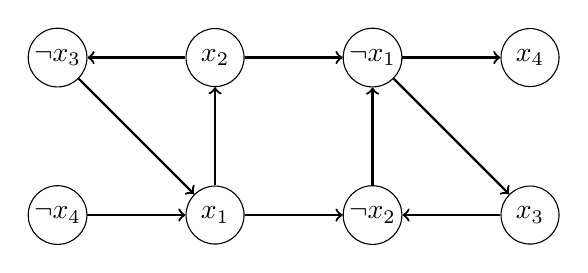
\begin{tikzpicture}[scale=1.0,minimum size=2pt]
\node[draw, circle, inner sep=1.3pt] (1) at (1,2) {$\lnot x_3$};
\node[draw, circle] (2) at (3,2) {$x_2$};
\node[draw, circle, inner sep=1.3pt] (3) at (1,0) {$\lnot x_4$};
\node[draw, circle] (4) at (3,0) {$x_1$};
\node[draw, circle, inner sep=1.3pt] (5) at (5,2) {$\lnot x_1$};
\node[draw, circle] (6) at (7,2) {$x_4$};
\node[draw, circle, inner sep=1.3pt] (7) at (5,0) {$\lnot x_2$};
\node[draw, circle] (8) at (7,0) {$x_3$};

\path[draw,thick,->] (1) -- (4);
\path[draw,thick,->] (4) -- (2);
\path[draw,thick,->] (2) -- (1);
\path[draw,thick,->] (3) -- (4);
\path[draw,thick,->] (2) -- (5);
\path[draw,thick,->] (4) -- (7);
\path[draw,thick,->] (5) -- (6);
\path[draw,thick,->] (5) -- (8);
\path[draw,thick,->] (8) -- (7);
\path[draw,thick,->] (7) -- (5);
\end{tikzpicture}
\end{center}
同じように$L_2$も次のように表現できます。
\\
\begin{center}
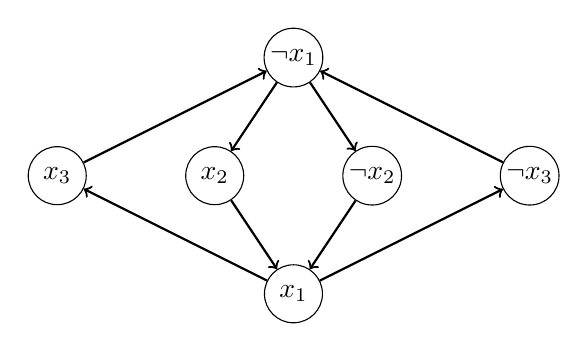
\begin{tikzpicture}[scale=1.0,minimum size=2pt]
\node[draw, circle] (1) at (1,2) {$x_3$};
\node[draw, circle] (2) at (3,2) {$x_2$};
\node[draw, circle, inner sep=1.3pt] (3) at (5,2) {$\lnot x_2$};
\node[draw, circle, inner sep=1.3pt] (4) at (7,2) {$\lnot x_3$};
\node[draw, circle, inner sep=1.3pt] (5) at (4,3.5) {$\lnot x_1$};
\node[draw, circle] (6) at (4,0.5) {$x_1$};

\path[draw,thick,->] (1) -- (5);
\path[draw,thick,->] (4) -- (5);
\path[draw,thick,->] (6) -- (1);
\path[draw,thick,->] (6) -- (4);
\path[draw,thick,->] (5) -- (2);
\path[draw,thick,->] (5) -- (3);
\path[draw,thick,->] (2) -- (6);
\path[draw,thick,->] (3) -- (6);
\end{tikzpicture}
\end{center}

グラフを用いて式が真となるように変数の値を割り当てることが可能かどうかを調べられます。
ある強連結成分に論理変数$x_i$とその否定$\lnot x_i$が同時に所属しなければ、
この式を成立させる組み合わせが存在するといえます。
逆に両ノードが同じ強連結成分に所属す
る時、その2つの変数は同時に満たされなければならず、
成立する組み合わせがないといえます。
この条件によって式 $L_1$ のグラフはその解が存在することがわかり、
$L_2$は成立する組み合わせがないことがわかります。

解が存在する場合は成分グラフをトポロジカルソートの逆順に見ていくことで、
変数の割り当てを求めることができます。
各ステップで、未処理成分に含まれる処理をしていきます。
ある成分をみて値が割り当て割れていなければ、
成分内の変数に値が割り当てられていない場合、
その値は成分内の値に従って決定します。
もし割り当てが決まっているならばなにもしません。

例えば、$L_1$のグラフのトポロジカルソート後の接続は以下のようになっていました。
\begin{center}
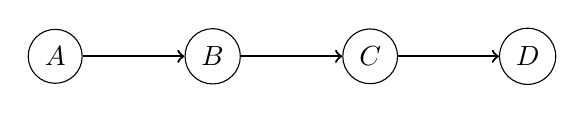
\begin{tikzpicture}[scale=1.0]
\node[draw, circle] (1) at (0,0) {$A$};
\node[draw, circle] (2) at (2,0) {$B$};
\node[draw, circle] (3) at (4,0) {$C$};
\node[draw, circle] (4) at (6,0) {$D$};

\path[draw,thick,->] (1) -- (2);
\path[draw,thick,->] (2) -- (3);
\path[draw,thick,->] (3) -- (4);
\end{tikzpicture}
\end{center}

各成分は次の通りです。
$A = \{\lnot x_4\}$,
$B = \{x_1, x_2, \lnot x_3\}$,
$C = \{\lnot x_1, \lnot x_2, x_3\}$,
$D = \{x_4\}$。

この解となる割り当てを決める時、
まず$x_4$がtrueとなる成分$D$を処理します。
その後、構成要素 $C$を処理し、$x_1$ と $x_2$ がfalse、$x_3$ がtrueとなります。

これで全ての論理変数に値が割り当てられたので、
残りの構成要素$A$と$B$は割り当てを変更しません。

このような割り当てができるのはグラフが特殊な構造だからです。
ノード$x_i$  からノード$x_j$  へ、
ノード$x_j$からノード$\lnot x_j$ へのパスがある場合、
ノード$x_i$ は決して真にはなりません。
この理由は、ノード
 $\lnot x_j$からノード$\lnot x_i$ そして $x_i$ and $x_j$  の両方が偽になるからです。

 \index{3SAT problem}

さらに難しい問題として、式の各部分が (ai ∨ bi ∨ ci ) のような形になる3-SAT
問題があります。ただしこの問題はNP困難であり、この問題を解く効率的なアルゴリズムは知られていない。
